%\documentclass[a4paper]{article}
\documentclass{aa}

\newcommand{\hi}{\mbox{H\,\sc{i}}}
\newcommand{\kms}{km\,s$^{-1}$}
\usepackage{graphicx}

\usepackage{txfonts}
\usepackage{natbib}
%\usvepackage[english]{babel}
%\usepackage[utf8]{inputenc}
%\usepackage{amsmath}
%\usepackage{graphicx}
%\usepackage[colorinlistoftodos]{todonotes}

\begin{document}

\title{An analysis of the energetics involved in the HI supershells}




\author{L. A. Suad\inst{1}, C. F. Caiafa\inst{1,2}, S. Cichowolski\inst{3}, \and E. M. Arnal\inst{1,4}}

\institute{Instituto Argentino de Radioastronomía (CCT-La Plata, CONICET; CICPBA), C.C. No. 5, 1894,Villa Elisa, Argentina.
  \and Facultad de Ingenier\'{i}a, Universidad de Buenos Aires (FIUBA), C.A.B.A, Argentina.
  \and Instituto de Astronom\'{i}a y F\'{i}sica del Espacio (CONICET-UBA), Cuidad Universitaria, C.A.B.A, Argentina. 
  \and Facultad de Ciencias Astron\'omicas y Geof\'{\i}sicas, Universidad Nacional de La Plata, La Plata, Argentina.
}
% * <lausuad@gmail.com> 2017-05-22T16:22:07.189Z:
%
% ^.




\date{\today}
%\maketitle
% * <lausuad@gmail.com> 2017-05-22T16:22:12.280Z:
%
% ^.

\abstract{}{}{}{}{} 



  \keywords{GS- shells 
                $\kappa$-mechanism --
                stability of gas spheres
               }

   \maketitle


\section{Introduction}\label{intro}


The interstellar medium (ISM) presents several features like bubbles, shells, supershells, worms that modifies the structure and dynamics of the Galaxy. In particular neutral hydrogen (\hi) Galactic supershells (GS) are arc-like structures, detected in a certain velocity range that could be surrounded, partially or completely, by walls of \hi\, emission. They are detected predominantly in the \hi\, emission distribution  although they can also be detected at other wavelengths (infrared, CO, optical). These are huge structures which radius varies from 100 to 500 pc according to \cite{sua14}.

The origin of these structures is currently a subject of debate. Given that about 70 \% of the massive stars in the Galaxy belongs to clusters or OB associations, the most probable mechanism for the GS formation could be the continuous energy injection from multiple massive stars \citep{nav16}. Other mechanisms have been proposed to explain its origin, for example the in-fall of high velocity clouds with the Galactic plane \citep{ten81}. One way of differentiating  which mechanism took place, it is to know its kinetic energy. To this end, it is necessary to know the mass of the structures.

Aca hay que describir un poco el catálogo (explicar que hay estructuras con 1, 2, y 3 cuadrantes llenos)

hay en el catalogo 308 con 4 cuadrantes llenos y 182 con 3 cuadrantes llenos

The goal of this paper is to have an estimation of the kinetic energy involved in the  GSs from the catalog of \cite{sua14}. To this end it is necessary to have a good estimation of the GSs masses. 

In this work we  have developed an algorithm that automatically detects the boundaries of supershells and calculates their associated masses. We applied the algorithm to the GSs cataloged in the paper of \cite{sua14}.

\section{Observations}

\hi\, data were retrieved form the Leiden-Argentine-Bonn (LAB) survey \citep{kal05}. This database has an angular resolution of 34', a velocity resolution of  1.3 \kms,  a channel separation of 1.03 \kms, and it covers the velocity range from $-400$ to $+450$ \kms. The entire database has been corrected for stray radiation \citep{kal05}.

  
\section{Estimation of GS's masses}

In this Section we describe the mechanisms used to estimate the amount of \hi\, mass contained in the GSs. 

As mentioned above, the GSs are  large voids  surrounded completely or partially by walls of \hi\, emission. A sketch of a prototypical feature is shown in Fig. \ref{sc}, along with a profile showing the different temperatures that characterizes each GS. Based on the hypothesis that before the structure was formed the \hi\, was uniformly distributed, we can assume that the excess mass in the shell should be equal to the mass missing in the void. 
Thus, we  can measure both, the excess mass of the \hi\, shell that borders the cavity, denoted by  $M_{\mathrm{HI}}^{\mathrm{shell}}$, and  the mass missing in the void, which we will refer to as the missing mass, $M_{\mathrm{HI}}^{\mathrm{miss}}$.
In an ideal case these two values should be exactly the same, however,
owing to  inhomogeneities present in the ISM where the structures are located, the estimated values do not always match. 

%that makes very difficult to delimited the shell (the void and the walls) this values do not always match. 





\begin{figure}
\centering
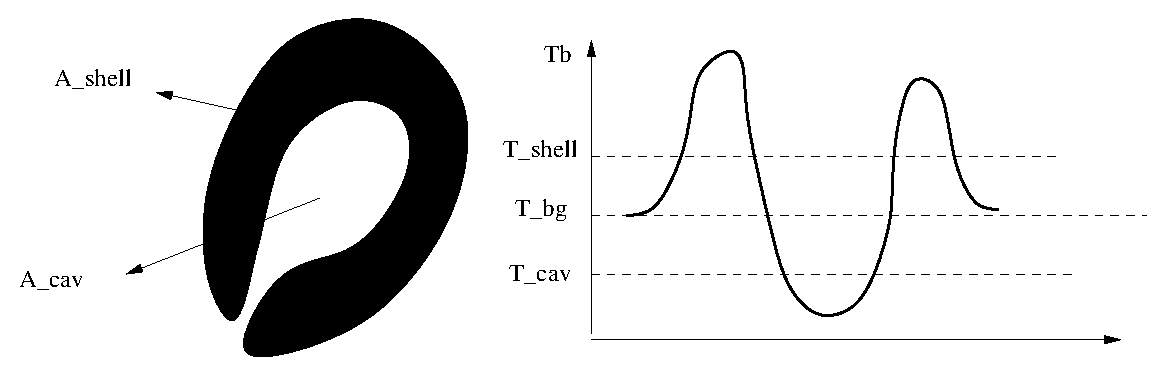
\includegraphics[width=9cm]{sc.eps}
\caption{}
\label{sc}
\end{figure}

Under the assumption that the \hi\, gas is optically thin, the neutral masses of an \hi\, structure located at a distance of $D$ kpc and  having an   angular size $\Omega_{\rm am2}$ arcmin$^2$ can be easily  estimated by

\begin{equation}
M_{\mbox{H\,\sc{i}}}(M_{\odot}) \approx 1.3 \times 10^{-3}\, D_{\rm kpc}^2\, \Delta {\rm v}_{\rm km\,s^{-1}} \, \int{\Delta T_{b} \, d\,\Omega_{\rm am2}}
\label{eq:masa}
\end{equation}

\noindent which gives an approximation to  an exact integral over velocity,  we just take $\Delta {\rm v}_{\rm km\,s^{-1}}$ as the velocity interval  over which the GS is visible.

To estimate the excess mass in the shell and the missing mass in the cavity, we define three temperatures that characterizes the structure: $T_{\rm cav}$ and $T_{\rm shell}$ as the average brightness temperature in the cavity and in the shell, respectively, and $T_{\rm bg}$ as the background temperature (see Fig. \ref{sc}).
Thus, from Eq. \ref{eq:masa} we obtain $M_{\mathrm{HI}}^{\mathrm{shell}}$ and $M_{\mathrm{HI}}^{\mathrm{miss}}$ replacing $\Delta T_{b}$ by ($T_{\rm shell} - T_{\rm bg}$) and ( $T_{\rm cav} -T_{\rm bg}$), respectively.

\subsection{Estimation by hand}\label{hand}

To estimate the neutral masses of a given structure it is necessary to first determine all the involved parameters: the distance, the velocity interval where the structure is observed, the three temperatures defined above, and the angular size of the shell and the cavity. 

As a first step, by inspecting the \hi\, data-cube, the velocity interval where the supershell is better observed is determined and used to create a velocity  averaged image. Secondly, this image is used to estimate the three temperatures and both angular areas.
Clearly, all these values have a large uncertainty, which must be taken into account in the value of the mass.
For instance, given the nonuniform background, the determination of the shell location is usually quite subjective and not easy.
To determine $T_{\rm bg}$ we consider the value  of the contour level defining the outer border of the \hi\, void, which represents the temperature of the neighboring gas. This contour is also used to  define  the  angular  extent  of  the  cavity and the inner border of the shell.

Taking into account all the errors involved, we can assume that the masses  calculated using 
Eq. \ref{eq:masa} have an error of not less than 50\%.




\subsection{Automatic algorithm}
\label{algorithm}




\section{Validation of the algorithm}

Since the goal of this paper is to determine  the kinetic energy stored in  all the Galactic supershell candidates having  four or three filled quadrants in the recently published catalogue of \citet{sua14}, we need first to be confident that the  masses obtained by the algorithm can be trusted.

To test the values yield by the algorithm, we have measured individually the masses of 92 GS belonging to the catalogue, 60 with four filled quadrants (group $A$ from hereon) and 32 with three filled quadrants (group $B$ from hereon).
It is important to mention that the 92 GS were randomly selected, so the sample 
contains  structures having  different shapes  and located in different regions of the outer part of the Galaxy (at both high and low Galactic latitudes and near the Galactic plane).

Following the procedure described in Section \ref{hand} and using Eq. \ref{eq:masa} we estimated the 92 excess and missing masses for structures of group $A$ and $B$ shown in Table \ref{massesA} and Table \ref{massesB}, respectively. The distance $d$, and the velocity interval where the GS is visible 
$\Delta {\rm v}_{\rm km\,s^{-1}}$ adopted for each structure were taken from the catalogue \citep{sua14}.

Figure aa and bb show a comparison between the shell masses, $M_{\mathrm{HI}}^{\mathrm{shell}}$,  and    the missing ones, $M_{\mathrm{HI}}^{\mathrm{miss}}$, obtained by hand and by the algorithm, for group $A$ and group $B$, respectively.
As can be seen, assuming an error of 50\% for all the estimations, the values obtained from both procedures agrees in a hh\% (group $A$) and ff\% (group $B$) of the structures.

aca va el motivo de las que no coinciden




 

%From Suad's catalog we can see that group {\it A} contains 308  and group {\it B} 182 supershell's candidates. 
%For each group we have selected  20 \% of the structures, that is, 62 GSs for group {\it A} and 36 for {\it B}. 


%Both, $d$,  $v_1$ and $v_2$ were taken form \cite{sua14}.



\begin{table*}
\caption{Shell and missing masses obtained for sample \it {A}. } 
\label{massesA}
\centering  
\begin{tabular}{l c c c c }
\hline \hline
   \,\,\, ID & $M_{\mathrm{HI}}^{\mathrm{shell}}$ (Hand)  &  $M_{\mathrm{HI}}^{\mathrm{miss}} $(Hand)& $M_{\mathrm{HI}}^{\mathrm{shell}}$ (Alg.)  &  $M_{\mathrm{HI}}^{\mathrm{miss}} $(Alg.)\\
  & $\times 10^4$\, M$_\odot$ &  $\times 10^4$\, M$_\odot$ & $\times 10^4$\, M$_\odot$ & $\times 10^4$\, M$_\odot$ \\
\hline
GS093-06-034	&	5.06	&	2.78	&	6.21	&	5.59	\\
GS100-06-019	&	5.16	&	2.70	&	1.48	&	1.48	\\
GS101-02-037	&	11.70	&	6.62	&	7.47	&	6.76	\\
GS101+29-026	&	5.93	&	4.96	&	8.10	&	8.10	\\
GS102-08-054	&	10.70	&	6.06	&	11.36	&	6.90	\\
GS104+03-038	&	6.20	&	3.90	&	5.85	&	5.85	\\
GS105-12-040	&	2.42	&	2.33	&	1.53	&	1.51	\\
GS107+02-069	&	7.14	&	4.40	&	2.47	&	2.47	\\
GS107+13-040	&	3.80	&	2.04	&	2.62	&	2.78	\\
GS108-03-022	&	8.31	&	5.23	&	9.79	&	9.79	\\
GS108+03-088	&	3.26	&	1.68	&	7.91	&	4.90	\\
GS113-01-075	&	9.10	&	4.69	&	8.69	&	8.70	\\
GS113-14-042	&	3.64	&	3.21	&	5.56	&	5.56	\\
GS114-03-054	&	1.86	&	0.96	&	5.97	&	5.97	\\
GS114-05-062	&	4.21	&	3.94	&	2.14	&	1.94	\\
GS115-05-054	&	2.24	&	1.80	&	1.99	&	2.01	\\
GS118+01-044	&	3.79	&	5.12	&	15.54	&	15.34	\\
GS119-04-058	&	7.10	&	4.86	&	9.82	&	9.89	\\
GS121-05-037	&	11.10	&	5.85	&	6.46	&	6.49	\\
GS122-02-077	&	33.80	&	25.00	&	4.66	&	4.30	\\
GS124-09-043	&	4.25	&	2.30	&	20.73	&	20.78	\\
GS129+05-061	&	21.10	&	10.50	&	5.73	&	3.97	\\
GS133-07-045	&	15.80	&	9.75	&	16.43	&	16.14	\\
GS135-09-056	&	5.44	&	4.77	&	13.88	&	13.87	\\
GS136-09-033	&	2.25	&	1.30	&	0.57	&	0.57	\\
GS137+03-063	&	4.24	&	2.24	&	5.51	&	5.51	\\
GS138+02-053	&	2.62	&	1.38	&	6.86	&	5.38	\\
GS140-03-079	&	29.70	&	25.10	&	57.83	&	57.84	\\
GS141-10-042	&	2.88	&	1.85	&	4.20	&	4.19	\\
GS144+08-031	&	6.51	&	3.50	&	5.34	&	5.34	\\
GS146-11-025	&	1.21	&	0.91	&	7.85	&	7.86	\\
GS146-11-045	&	0.41	&	0.22	&	2.38	&	0.72	\\
GS153+02-047	&	2.46	&	1.40	&	7.79	&	7.74	\\
GS164+00-021	&	2.88	&	3.07	&	5.81	&	6.50	\\
GS195+28+014	&	0.31	&	0.24	&	0.48	&	0.48	\\
GS198-01+035	&	3.57	&	2.03	&	5.80	&	5.82	\\
GS199-13+025	&	0.54	&	0.27	&	0.94	&	0.79	\\
GS201-23+025	&	0.40	&	0.21	&	0.17	&	0.14	\\
GS202+10+014	&	0.64	&	0.37	&	0.17	&	0.17	\\
GS221-03+045	&	2.75	&	1.76	&	4.83	&	4.87	\\
GS222+13+026	&	0.56	&	0.40	&	1.09	&	1.09	\\
GS227+05+051	&	0.95	&	0.63	&	2.00	&	2.00	\\
GS229+03+073	&	2.22	&	1.22	&	3.05	&	3.05	\\
GS230-06+040	&	6.35	&	3.55	&	18.74	&	18.91	\\
GS232+02+081	&	3.26	&	1.72	&	2.70	&	2.76	\\
GS239-02+068	&	7.21	&	4.69	&	23.20	&	19.29	\\
GS240+00+035	&	0.48	&	0.47	&	0.32	&	0.32	\\
GS240+05+033	&	0.53	&	0.40	&	0.57	&	0.57	\\
GS246+07+048	&	0.59	&	0.57	&	1.05	&	1.05	\\
GS247+00+086	&	7.47	&	3.75	&	6.44	&	5.37	\\
GS253-12+053	&	4.56	&	2.95	&	0.66	&	0.59	\\
GS253+07+062	&	10.00	&	5.18	&	8.34	&	8.33	\\
GS256-16+055	&	1.17	&	0.77	&	0.55	&	0.55	\\
GS257+00+067	&	2.01	&	1.18	&	2.30	&	2.31	\\
GS259-08+090	&	10.90	&	6.65	&	19.86	&	19.86	\\
GS260-04+081	&	3.72	&	3.70	&	2.37	&	2.35	\\
GS261-03+055	&	2.49	&	1.65	&	3.10	&	3.10	\\
GS263+10+020	&	1.33	&	1.39	&	2.20	&	2.19	\\
GS265-06+082	&	12.80	&	6.75	&	6.56	&	6.36	\\
GS269+04+044	&	6.09	&	3.15	&	8.21	&	8.21	\\
\hline
\end{tabular}
\end{table*}

\begin{table*}
\caption{Shell and missing masses obtained for sample \it {B}.} 
\label{massesB}
\centering  
\begin{tabular}{l c c c c }
\hline \hline
   \,\,\, ID & $M_{\mathrm{HI}}^{\mathrm{shell}}$ (Hand)  &  $M_{\mathrm{HI}}^{\mathrm{miss}} $(Hand)& $M_{\mathrm{HI}}^{\mathrm{shell}}$ (Alg.)  &  $M_{\mathrm{HI}}^{\mathrm{miss}} $(Alg.)\\
  & $\times 10^4$\, M$_\odot$ &  $\times 10^4$\, M$_\odot$ & $\times 10^4$\, M$_\odot$ & $\times 10^4$\, M$_\odot$ \\
\hline
  GS089-21-025*   	&	3.26	&	4.05	&	6.18	&	7.00	\\
  GS093-14-021*   	&	8.88	&	4.50	&	28.37	&	28.14	\\
  GS093+11-034*   	&	2.54	&	1.28	&	1.88	&	1.88	\\
  GS098-25-018*   	&	1.08	&	1.08	&	1.47	&	1.16	\\
  GS098+24-032   	&	0.96	&	0.81	&	2.58	&	2.58	\\
  GS100+09-040*   	&	5.34	&	2.99	&	8.14	&	8.14	\\
  GS101-13-056*   	&	24.00	&	16.90	&	18.69	&	18.68	\\
  GS105-03-061   	&	22.40	&	12.40	&	5.34	&	3.93	\\
  GS108+00-075*   	&	4.67	&	2.86	&	9.47	&	9.48	\\
  GS109+06-032   	&	2.50	&	1.65	&	3.94	&	3.97	\\
  GS109+16-033*   	&	6.54	&	7.24	&	6.76	&	6.75	\\
  GS110-04-067   	&	7.80	&	7.15	&	5.74	&	2.79	\\
  GS116-06-042*   	&	2.49	&	1.89	&	5.95	&	5.97	\\
  GS117+08-076*   	&	5.49	&	3.92	&	17.51	&	17.62	\\
  GS120+08-028   	&	3.20	&	1.97	&	2.19	&	2.15	\\
  GS120+16-067*   	&	6.54	&	3.79	&	3.57	&	3.59	\\
  GS130+00-068*   	&	1.52	&	0.83	&	0.21	&	0.16	\\
  GS139+06-054*   	&	3.20	&	0.87	&	2.39	&	2.17	\\
  GS142-01-057   	&	2.03	&	1.26	&	2.67	&	2.67	\\
  GS142-01-057   	&	7.86	&	10.10	&	2.67	&	2.67	\\
  GS153-10-026*   	&	1.55	&	1.55	&	0.42	&	0.42	\\
  GS153-10-026*   	&	1.78	&	1.01	&	0.42	&	0.42	\\
  GS161+03-036   	&	34.50	&	19.40	&	28.47	&	21.79	\\
  GS202+05+031   	&	1.74	&	0.92	&	8.99	&	8.97	\\
  GS218-05+037*   	&	0.80	&	0.80	&	3.96	&	3.96	\\
  GS224-18+036   	&	0.30	&	0.22	&	1.01	&	1.01	\\
  GS240-13+064*   	&	1.60	&	1.45	&	2.33	&	2.33	\\
  GS246-05+086   	&	2.67	&	1.94	&	1.14	&	1.21	\\
  GS247+06+055*   	&	0.88	&	1.12	&	3.07	&	3.08	\\
  GS252-04+074*   	&	11.40	&	7.82	&	47.88	&	47.82	\\
  GS257-25+030*   	&	0.58	&	0.30	&	0.42	&	0.42	\\
  GS257+09+037   	&	4.99	&	2.86	&	5.33	&	5.35	\\
  GS262-09+048*   	&	5.52	&	3.95	&	3.27	&	3.41	\\
  GS263-08+068*   	&	13.70	&	11.90	&	9.99	&	10.00	\\
  GS264-04+044   	&	3.90	&	2.23	&	2.42	&	2.42	\\
GS103+07-018*   	&	8.54	&	8.28	&	21.58	&	21.60	\\
\hline
\end{tabular}
\end{table*}


\section{Kinetic energy estimation}






\bibliographystyle{aa} 
\bibliography{bibliografia}
  
 \IfFileExists{\jobname.bbl}{}
{\typeout{}
\typeout{****************************************************}
\typeout{****************************************************}
\typeout{** Please run "bibtex \jobname' ' to optain}
\typeout{** the bibliography and then re-run LaTeX}
\typeout{** twice to fix the references!}
\typeout{****************************************************}
\typeout{****************************************************}
\typeout{}
}



\begin{acknowledgements}
      
\end{acknowledgements}



%Comments can be added to the margins of the document using the \todo{Here's a comment in the margin!} todo command, as shown in the example on the right. You can also add inline comments:

%\todo[inline, color=green!40]{This is an inline comment.}



%\subsection{How to Make Tables}



%\begin{table}
%\centering
%\begin{tabular}{l|r}
%Item & Quantity \\\hline
%Widgets & 42 \\
%Gadgets & 13
%\end{tabular}
%\caption{\label{tab:widgets}An example table.}
%\end{table}


%\noindent where $N_{\mathrm{HI}}$  is the \hi\, column density and $A_{\mathrm{HI}}$ is the area of the supershell, $A_{\mathrm{HI}} = \Omega_{\mathrm{HI}} d^2$, where $\Omega_{\mathrm{HI}}$ is the solid angle covered by the structure and $d$ is the distance to the Sun.





%\noindent $v_1$ and $v_2$  are the velocity interval where the structure is detected and the mean brightness temperature $\Delta T_b$ is defined as $\Delta T_b = | T_{cav}-T_{bg}|$, where $T_{cav}$ refers to the mean 
%&brightness temperature of the HI cavity to measure $M_{\mathrm{HI}}^{\mathrm{miss}}$ (or the mean 
%brightness temperature of the shell to measure $M_{\mathrm{HI}}^{\mathrm{ring}}$, depending on which mass we are estimating), and $T_{bg}$
%corresponds to the temperature of the contour level defining the outer border of the HI minimum and represents the temperature of the neighboring gas. 
%To  define  the  angular  extent  of  the  HI  cavity,  we  adopt the  first  non closed  contour  line  defining  the  void.
%As said above, it is hard to estimate the limits of the shell (or the void) not only because the inhomogeneities of the ISM but also because of huge quantity of \hi\, present in the Galaxy. 




\end{document}